%%%%%%%% ICML 2027 EXAMPLE LATEX SUBMISSION FILE %%%%%%%%%%%%%%%%%

\documentclass{article}

% Recommended, but optional, packages for figures and better typesetting:
\usepackage{microtype}
\usepackage{graphicx}
\usepackage{subcaption}
\usepackage{booktabs} % for professional tables

% hyperref makes hyperlinks in the resulting PDF.
% If your build breaks (sometimes temporarily if a hyperlink spans a page)
% please comment out the following usepackage line and replace
% \usepackage{icml2027} with \usepackage[nohyperref]{icml2027} above.
\usepackage{hyperref}


% Attempt to make hyperref and algorithmic work together better:
\newcommand{\theHalgorithm}{\arabic{algorithm}}

% Use the following line for the initial blind version submitted for review:
\usepackage{icml2027}

% For preprint, use
% \usepackage[preprint]{icml2027}

% If accepted, instead use the following line for the camera-ready submission:
% \usepackage[accepted]{icml2027}

\usepackage{amsmath}
\usepackage{amssymb}
\usepackage{mathtools}
\usepackage{amsthm}


% if you use cleveref..
\usepackage[capitalize,noabbrev]{cleveref}

%%%%%%%%%%%%%%%%%%%%%%%%%%%%%%%%
% THEOREMS
%%%%%%%%%%%%%%%%%%%%%%%%%%%%%%%%
\theoremstyle{plain}
\newtheorem{theorem}{Theorem}[section]
\newtheorem{proposition}[theorem]{Proposition}
\newtheorem{lemma}[theorem]{Lemma}
\newtheorem{corollary}[theorem]{Corollary}
\theoremstyle{definition}
\newtheorem{definition}[theorem]{Definition}
\newtheorem{assumption}[theorem]{Assumption}
\theoremstyle{remark}
\newtheorem{remark}[theorem]{Remark}

% Todonotes is useful during development; simply uncomment the next line
%    and comment out the line below the next line to turn off comments
%\usepackage[disable,textsize=tiny]{todonotes}
\usepackage[textsize=tiny]{todonotes}

% The \icmltitle you define below is probably too long as a header.
% Therefore, a short form for the running title is supplied here:
\icmltitlerunning{Submission and Formatting Instructions for ICML 2027}

\begin{document}

\twocolumn[
  \icmltitle{Submission and Formatting Instructions for \\
    International Conference on Machine Learning (ICML 2027)}

  % It is OKAY to include author information, even for blind submissions: the
  % style file will automatically remove it for you unless you've provided
  % the [accepted] option to the icml2027 package.

  % List of affiliations: The first argument should be a (short) identifier you
  % will use later to specify author affiliations Academic affiliations
  % should list Department, University, City, Region, Country Industry
  % affiliations should list Company, City, Region, Country

  % You can specify symbols, otherwise they are numbered in order. Ideally, you
  % should not use this facility. Affiliations will be numbered in order of
  % appearance and this is the preferred way.
  \icmlsetsymbol{equal}{*}

  \begin{icmlauthorlist}
    \icmlauthor{Firstname1 Lastname1}{equal,yyy}
    \icmlauthor{Firstname2 Lastname2}{equal,yyy,comp}
    \icmlauthor{Firstname3 Lastname3}{comp}
    \icmlauthor{Firstname4 Lastname4}{sch}
    \icmlauthor{Firstname5 Lastname5}{yyy}
    \icmlauthor{Firstname6 Lastname6}{sch,yyy,comp}
    \icmlauthor{Firstname7 Lastname7}{comp}
    %\icmlauthor{}{sch}
    \icmlauthor{Firstname8 Lastname8}{sch}
    \icmlauthor{Firstname8 Lastname8}{yyy,comp}
    %\icmlauthor{}{sch}
    %\icmlauthor{}{sch}
  \end{icmlauthorlist}

  \icmlaffiliation{yyy}{Department of XXX, University of YYY, Location, Country}
  \icmlaffiliation{comp}{Company Name, Location, Country}
  \icmlaffiliation{sch}{School of ZZZ, Institute of WWW, Location, Country}

  \icmlcorrespondingauthor{Firstname1 Lastname1}{first1.last1@xxx.edu}
  \icmlcorrespondingauthor{Firstname2 Lastname2}{first2.last2@www.uk}

  % You may provide any keywords that you find helpful for describing your
  % paper; these are used to populate the "keywords" metadata in the PDF but
  % will not be shown in the document
  \icmlkeywords{Machine Learning, ICML}

  \vskip 0.3in
]

% this must go after the closing bracket ] following \twocolumn[ ...

% This command actually creates the footnote in the first column listing the
% affiliations and the copyright notice. The command takes one argument, which
% is text to display at the start of the footnote. The \icmlEqualContribution
% command is standard text for equal contribution. Remove it (just {}) if you
% do not need this facility.

% Use ONE of the following lines. DO NOT remove the command.
% If you have no special notice, KEEP empty braces:
\printAffiliationsAndNotice{}  % no special notice (required even if empty)
% Or, if applicable, use the standard equal contribution text:
% \printAffiliationsAndNotice{\icmlEqualContribution}

\begin{abstract}
  This document provides a basic paper template and submission guidelines.
  Abstracts must be a single paragraph, ideally between 4--6 sentences long.
  Gross violations will trigger corrections at the camera-ready phase.
\end{abstract}

\section{Introduction}
Skills can augment LLM-based agents handle complex tasks by following procedure guidelines,
leveraging external tools, and utilizing domain knowledge~\cite{xxx}. 
Various skills, whether manually created by using human expertise~\cite{xxx} or generated automatically through skill generation~\cite{xxx} and evolution~\cite{xxx} during task executions, have been developed by various skill providers and distributed in various skill repositories. 
For example, some well-known agent companies, such as Anthropic~\cite{xxx} and OpenAI~\cite{xxx}, have been actively developing and publishing large amount of skills for various tasks of various domains,
such as coding and document processing. 
% Skill providers have been actively developing large amount of skills specially designedfor various tasks and domains, and publishing them online dispersedly across various repositories. 
% For example, Anthropic~\cite{xx} published xxx.
Applying appropriate skills that match the requirements of a given task is crucial for agents to achieve high performance.
However, customized agent systems, which also requires specially designed skills for specific domains, e.g., healthcare, need spend much effort looking for suitable skills from diverse repositories.
The dispersed nature of skill repositories make it challenging for these agent systems to maintain and utilize appropriate skills.
Maintaining a unified skill library can alleviate the burden of skill management and facilitate the development of customized agent systems.

However, building an unified skill library that is reliable and efficiently usable can be challenging due to the following reasons.
1) \textbf{Cross-repository conflicts}: skills of similar tasks usually have format and content conflicts when they are from different repositories developed by different providers. 
These conflicts, which arise from various factors, such as different design principles of providers and task scenarios, need to be properly resolved to ensure skill compatibility and usability.
2) \textbf{Task-skill matching biases}: locating appropriate skills among tens of thousands of skills in the library for a given task \textcolor{blue}{is prone to errors and can be costly.
xxxxxxxxxxxxxxxxxxxxxx.}
3) \textbf{Skill exposure overhead}: compared to the traditional approach of exposing skill metadata in the conversation context for the awareness of skill information, calling a large-scale skill library requires careful design of usage interfaces to avoid overwhelming the agent with excessive information, while ensuring that the agent can effectively utilize the skills.
These challenges directly impact the quality of skills and the effective and efficient usage of them. 


Recent studies have addressed important aspects of skill library construction and usage.
SkillNet~\cite{liang2026skillnet} organizes and evaluates skills from heterogeneous sources, while SkillCorpus~\cite{wang2026skillcorpus} combines community skill curation with retrieval and downstream evaluation.
For large-scale skill selection, SkillRouter~\cite{zheng2026skillrouter} develops a content-aware retrieval and reranking pipeline.
Building on these advances, we investigate conflict-aware consolidation, task-oriented indexing, and controlled skill exposure as coordinated construction and usage protocols for a unified skill library.

In this study, we systematically develop construction and usage protocols for a reliable and efficient unified skill library. 
First, to resolve skill conflicts from different repositories, we finalize skills into three types, namely individual, authentic, and combined, which correspond different levels of conflicts. 
Conditioned on these types, we cluster skills into non-overlapping groups based on their task similarity and handle conflicts within each group.
As a result, a finalized skill are considered to be compatible with others and can be reliably used by agents.
% We identify skill clusters around these types, and handle conflicts within each cluster. 
% Each individual skill is an originally independent one that is considered not to intersect with others. 
% A authentic skill is the leading copy of a cluster of same skills of different versions.
% A combined skill is a synthesized version created by merging multiple related skills.
Second, to facilitate finding skills for a given task, we design a hierarchical indexing structure driven around tasks for all finalized skills.
We classify skills first by domains and then by task families and file per-skill cards containing task-specific metadata.
Given a task query, this hierarchical indexing allows for a lightweight matching within a task-related, narrowed skill set, which has been efficiently filtered out with awareness to task-skill semantics, and therefore has less risk of matching biases.
\textcolor{blue}{About updates tonew skills....}
%  of task-can support efficient semantic-aware filtering of skill sets, which can reduce the risk of matching biases, and which has been semantically filtered  which is efficient and can reduce the risk of matching biases.
Third, to regulate the exposure of skill information to agents, we design the usage interfaces as simply two functions, namely \texttt{find\_skills} and \texttt{load\_skill}.
The two functions support the use of SkillLib in all scenarios without proactively exposing skill metadata in the conversation context, which can therefore avoid overwhelming the agent with excessive information while ensuring effective utilization of skills. 

Using the above protocols, we generates a unified, large-scale skill library, named \textbf{SkillLib}. 
We collect agent skills from high-reputation repositories of various providers and consolidate them into a single, extendable library. 
We implement SkillLib as an independent package that can be integrated seamlessly into an existing agent system. 
The evaluation results on various xxxxxxxxxxxxxxx. 


The major contributions of this study are summarized as follows. 
\begin{itemize}
  \item xxx
  \item xxx
  \item xxx
\end{itemize}


\section{Related Work}\label{sec:relatedWork}

\subsection{Agent Skill Acquisition and Library Consolidation}
Reusable skills enable agents to retain procedural knowledge across tasks.
Voyager~\cite{wang2023voyager} provides an early example by accumulating executable skills through open-ended exploration in Minecraft.
Agent Workflow Memory~\cite{wang2025awm} extends experience reuse to web navigation by inducing reusable workflows from offline demonstrations or online interactions.
Agent Skill Induction~\cite{wang2025asi} further represents web skills as programs that can be verified and adapted during execution.
These approaches primarily acquire skills within an agent's task environment; SkillLib addresses the subsequent integration of independently authored skills from multiple repositories.

Closer to our setting, SkillNet~\cite{liang2026skillnet} provides an infrastructure for creating, evaluating, and connecting skills through a unified ontology.
Its curation pipeline combines deduplication and quality filtering with explicit similarity, composition, and dependency relations.
SkillCorpus~\cite{wang2026skillcorpus} directly studies the consolidation of the open skill ecosystem, combining exact and semantic deduplication, quality assessment, and a retrieval-and-selection stack with evaluation on real agent tasks.
SkillLib places conflict handling at the center of this consolidation problem: its individual, authentic, and combined skill types distinguish preservation of independent skills, selection of a canonical version, and synthesis of related procedures.
This focus makes the handling of competing versions and overlapping instructions an explicit library-construction decision, alongside the downstream retrieval and access protocols.

\subsection{Task-Aware Skill Retrieval and Routing}
Large tool inventories motivated retrieval before the emergence of community skill libraries.
ToolLLM~\cite{qin2024toolllm} couples a large API collection with a neural retriever that identifies candidate APIs for an instruction.
AnyTool~\cite{du2024anytool} introduces hierarchical API discovery through category- and tool-level agents, establishing coarse-to-fine search as a precedent for scaling capability selection.
The representation being searched also matters: Tool-REX~\cite{lu2026toolrex} enriches heterogeneous tool documentation with structured fields and trains dedicated retrieval and reranking models.
These studies motivate both hierarchical organization and informative task-specific representations, although their retrieval units are API tools.

SkillRouter~\cite{zheng2026skillrouter} examines skill selection more directly, showing that names and descriptions can omit discriminative information contained in skill bodies.
Its body-aware retrieval and reranking pipeline addresses confusion among heavily overlapping skills at registry scale.
SkillFlow~\cite{li2026skillflow} progressively filters community skills through dense retrieval, two reranking stages, and LLM selection; its downstream results also show that retrieval gains depend on corpus coverage and executable skill content.
AgentSkillOS~\cite{li2026agentskillos} takes a structural approach, recursively organizing skills into a capability tree and composing retrieved skills into directed acyclic execution graphs.
SkillNet-Fabric~\cite{liang2026skillnet} further guides skill-set selection with task-specific Wikis built from skill contracts and relation-expanded candidates.
SkillLib organizes the outputs of conflict-aware consolidation into a domain--task-family hierarchy, with task-specific cards supporting matching within narrowed candidate sets.
This connects the skill artifacts produced during library construction to task-level candidate filtering and a separate loading interface.
SkillRouter's findings make the procedural information retained in these cards a central consideration in this design.

\subsection{Context-Efficient Skill Discovery and On-Demand Loading}
Capability access must balance informative selection with the context consumed by exposing available tools or skills.
ToolGen~\cite{wang2025toolgen} addresses this constraint by encoding tools as dedicated tokens and learning to generate tool identifiers and arguments, moving tool knowledge into model parameters.
External discovery offers another approach: MCP-Zero~\cite{fei2025mcpzero} lets agents identify capability gaps and request tools on demand through hierarchical server--tool routing, providing a direct precedent for agent-initiated capability acquisition.

ToolScope~\cite{liu2026toolscope} connects redundancy reduction to context control by merging semantically equivalent tools, auditing proposed merges, and retrieving a compact toolset for each query.
It is particularly relevant to SkillLib's joint treatment of consolidation and exposure, while operating on function signatures and tool descriptions rather than procedural skill packages.
Graph-of-Skills~\cite{liu2026graphskills} further shows why relevance filtering alone can be insufficient: it retrieves dependency-aware skill bundles and loads their content within a context budget to recover prerequisites that semantic search can miss.
SkillLib adopts a complementary access protocol: \texttt{find\_skills} exposes task-relevant candidates, and \texttt{load\_skill} supplies selected skill instructions on demand, without placing the entire library's metadata in the initial conversation context.
This protocol applies on-demand discovery and loading to the skill artifacts produced by consolidation, connecting context control to how the library is constructed and indexed.

\section{Background}

\section{Method}\label{sec:method}
\subsection{Overview}

SkillLib combines library construction with on-demand skill access.
\Cref{fig:lib-construction} summarizes conflict resolution, hierarchical indexing, and skill-card generation.
\Cref{fig:lib-usage} illustrates how an agent discovers relevant skill cards with \texttt{find\_skills} and retrieves the selected skill with \texttt{load\_skill}.

\begin{figure*}[t]
  \centering
  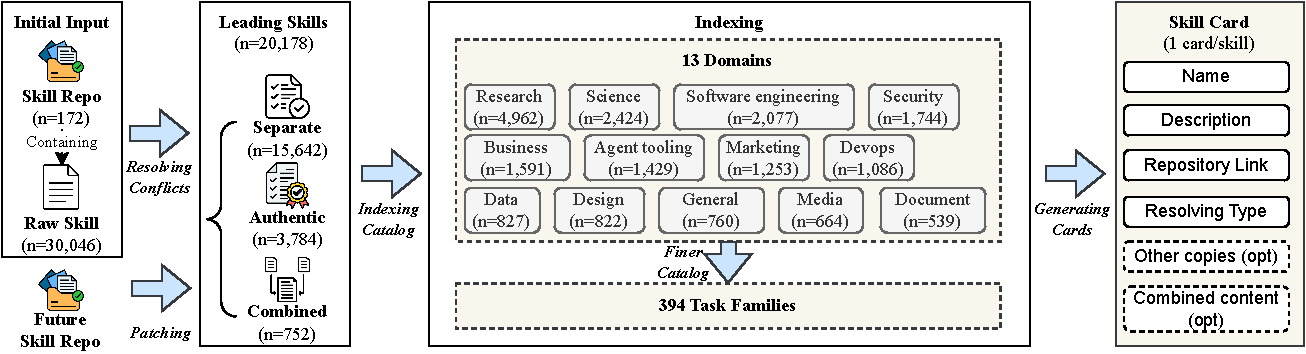
\includegraphics[width=\textwidth]{fig/libConstruction.pdf}
  \caption{Construction of SkillLib. Skills collected from multiple repositories undergo conflict resolution to produce leading skills, which are organized by domain and task family. Each skill receives a card containing its metadata and repository link. New repositories can be incorporated through subsequent updates.}
  \label{fig:lib-construction}
\end{figure*}

\begin{figure}[t]
  \centering
  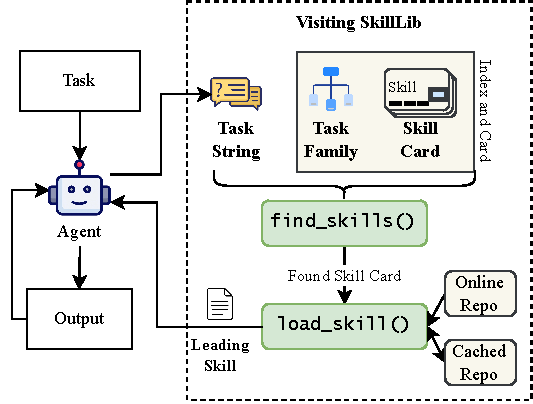
\includegraphics[width=\linewidth]{fig/libUsage.pdf}
  \caption{On-demand access to SkillLib. Given a task, the agent calls \texttt{find\_skills} to discover relevant skill cards through the hierarchical index, then calls \texttt{load\_skill} to retrieve a leading skill from an online or cached repository.}
  \label{fig:lib-usage}
\end{figure}

\section{Result}\label{sec:result}
\subsection{Experimental Setup}
\paragraph{Benchmarks.}
\paragraph{Metrics.}
\paragraph{Baselines.}
\paragraph{Running Details.}

\subsection{Main Results}

\section{Conclusion and Limitations}



\subsection{Algorithms}

If you are using \LaTeX, please use the ``algorithm'' and ``algorithmic''
environments to format pseudocode. These require the corresponding stylefiles,
algorithm.sty and algorithmic.sty, which are supplied with this package.
\cref{alg:example} shows an example.

\begin{algorithm}[tb]
  \caption{Bubble Sort}
  \label{alg:example}
  \begin{algorithmic}
    \STATE {\bfseries Input:} data $x_i$, size $m$
    \REPEAT
    \STATE Initialize $noChange = true$.
    \FOR{$i=1$ {\bfseries to} $m-1$}
    \IF{$x_i > x_{i+1}$}
    \STATE Swap $x_i$ and $x_{i+1}$
    \STATE $noChange = false$
    \ENDIF
    \ENDFOR
    \UNTIL{$noChange$ is $true$}
  \end{algorithmic}
\end{algorithm}


\subsection{Tables}

You may also want to include tables that summarize material. Like figures,
these should be centered, legible, and numbered consecutively. However, place
the title \emph{above} the table with at least 0.1~inches of space before the
title and the same after it, as in \cref{sample-table}. The table title should
be set in 9~point type and centered unless it runs two or more lines, in which
case it should be flush left.

% Note use of \abovespace and \belowspace to get reasonable spacing
% above and below tabular lines.

\begin{table}[t]
  \caption{Classification accuracies for naive Bayes and flexible
    Bayes on various data sets.}
  \label{sample-table}
  \begin{center}
    \begin{small}
      \begin{sc}
        \begin{tabular}{lcccr}
          \toprule
          Data set  & Naive         & Flexible      & Better?  \\
          \midrule
          Breast    & 95.9$\pm$ 0.2 & 96.7$\pm$ 0.2 & $\surd$  \\
          Cleveland & 83.3$\pm$ 0.6 & 80.0$\pm$ 0.6 & $\times$ \\
          Glass2    & 61.9$\pm$ 1.4 & 83.8$\pm$ 0.7 & $\surd$  \\
          Credit    & 74.8$\pm$ 0.5 & 78.3$\pm$ 0.6 &          \\
          Horse     & 73.3$\pm$ 0.9 & 69.7$\pm$ 1.0 & $\times$ \\
          Meta      & 67.1$\pm$ 0.6 & 76.5$\pm$ 0.5 & $\surd$  \\
          Pima      & 75.1$\pm$ 0.6 & 73.9$\pm$ 0.5 &          \\
          Vehicle   & 44.9$\pm$ 0.6 & 61.5$\pm$ 0.4 & $\surd$  \\
          \bottomrule
        \end{tabular}
      \end{sc}
    \end{small}
  \end{center}
  \vskip -0.1in
\end{table}


\subsection{Theorems and Such}
The preferred way is to number definitions, propositions, lemmas, etc.
consecutively, within sections, as shown below.
\begin{definition}
  \label{def:inj}
  A function $f:X \to Y$ is injective if for any $x,y\in X$ different, $f(x)\ne
    f(y)$.
\end{definition}
Using \cref{def:inj} we immediate get the following result:
\begin{proposition}
  If $f$ is injective mapping a set $X$ to another set $Y$,
  the cardinality of $Y$ is at least as large as that of $X$
\end{proposition}
\begin{proof}
  Left as an exercise to the reader.
\end{proof}
\cref{lem:usefullemma} stated next will prove to be useful.
\begin{lemma}
  \label{lem:usefullemma}
  For any $f:X \to Y$ and $g:Y\to Z$ injective functions, $f \circ g$ is
  injective.
\end{lemma}
\begin{theorem}
  \label{thm:bigtheorem}
  If $f:X\to Y$ is bijective, the cardinality of $X$ and $Y$ are the same.
\end{theorem}
An easy corollary of \cref{thm:bigtheorem} is the following:
\begin{corollary}
  If $f:X\to Y$ is bijective,
  the cardinality of $X$ is at least as large as that of $Y$.
\end{corollary}
\begin{assumption}
  The set $X$ is finite.
  \label{ass:xfinite}
\end{assumption}
\begin{remark}
  According to some, it is only the finite case (cf. \cref{ass:xfinite}) that
  is interesting.
\end{remark}
%restatable

\subsection{Citations and References}

Please use APA reference format regardless of your formatter or word processor.
If you rely on the \LaTeX\/ bibliographic facility, use \texttt{natbib.sty} and
\texttt{icml2027.bst} included in the style-file package to obtain this format.

Citations within the text should include the authors' last names and year. If
the authors' names are included in the sentence, place only the year in
parentheses, for example when referencing Arthur Samuel's pioneering work
\yrcite{Samuel59}. Otherwise place the entire reference in parentheses with the
authors and year separated by a comma \cite{Samuel59}. List multiple references
separated by semicolons \cite{kearns89,Samuel59,mitchell80}. Use the `et~al.'
construct only for citations with three or more authors or after listing all
authors to a publication in an earlier reference \cite{MachineLearningI}.

Authors should cite their own work in the third person in the initial version
of their paper submitted for blind review. Please refer to \cref{author info}
for detailed instructions on how to cite your own papers.

Use an unnumbered first-level section heading for the references, and use a
hanging indent style, with the first line of the reference flush against the
left margin and subsequent lines indented by 10 points. The references at the
end of this document give examples for journal articles \cite{Samuel59},
conference publications \cite{langley00}, book chapters \cite{Newell81}, books
\cite{DudaHart2nd}, edited volumes \cite{MachineLearningI}, technical reports
\cite{mitchell80}, and dissertations \cite{kearns89}.


\section*{Accessibility}

Authors are kindly asked to make their submissions as accessible as possible
for everyone including people with disabilities and sensory or neurological
differences. Tips of how to achieve this and what to pay attention to will be
provided on the conference website \url{http://icml.cc/}.

\section*{Software and Data}

If a paper is accepted, we strongly encourage the publication of software and
data with the camera-ready version of the paper whenever appropriate. This can
be done by including a URL in the camera-ready copy. However, \textbf{do not}
include URLs that reveal your institution or identity in your submission for
review. Instead, provide an anonymous URL or upload the material as
``Supplementary Material'' into the OpenReview reviewing system. Note that
reviewers are not required to look at this material when writing their review.

% Acknowledgements should only appear in the accepted version.
% \section*{Acknowledgements}

\section*{AI Use Statement}

Authors are \textbf{required} to include a statement describing how AI tools,
such as large language models (LLMs), were used in the research and in the
preparation of the paper. The statement does not count toward the page limit.
It should be short, typically a few sentences, and must not exceed one page.
Authors remain fully responsible for the entire content of the paper,
including any text, code, proofs or figures produced with the help of AI
tools, and LLMs cannot be listed as authors. Disclosing the use of AI tools
will not by itself count against a submission.


\section*{Impact Statement}

Authors are \textbf{required} to include a statement of the potential broader
impact of their work, including its ethical aspects and future societal
consequences. This statement should be in an unnumbered section at the end of
the paper (co-located with Acknowledgements -- the two may appear in either
order, but both must be before References), and does not count toward the paper
page limit. In many cases, where the ethical impacts and expected societal
implications are those that are well established when advancing the field of
Machine Learning, substantial discussion is not required, and a simple
statement such as the following will suffice:

``This paper presents work whose goal is to advance the field of Machine
Learning. There are many potential societal consequences of our work, none
which we feel must be specifically highlighted here.''

The above statement can be used verbatim in such cases, but we encourage
authors to think about whether there is content which does warrant further
discussion, as this statement will be apparent if the paper is later flagged
for ethics review.

% In the unusual situation where you want a paper to appear in the
% references without citing it in the main text, use \nocite
\nocite{langley00}

\bibliography{example_paper}
\bibliographystyle{icml2027}

%%%%%%%%%%%%%%%%%%%%%%%%%%%%%%%%%%%%%%%%%%%%%%%%%%%%%%%%%%%%%%%%%%%%%%%%%%%%%%%
%%%%%%%%%%%%%%%%%%%%%%%%%%%%%%%%%%%%%%%%%%%%%%%%%%%%%%%%%%%%%%%%%%%%%%%%%%%%%%%
% APPENDIX
%%%%%%%%%%%%%%%%%%%%%%%%%%%%%%%%%%%%%%%%%%%%%%%%%%%%%%%%%%%%%%%%%%%%%%%%%%%%%%%
%%%%%%%%%%%%%%%%%%%%%%%%%%%%%%%%%%%%%%%%%%%%%%%%%%%%%%%%%%%%%%%%%%%%%%%%%%%%%%%
\newpage
\appendix
\onecolumn
\section{You \emph{can} have an appendix here.}

You can have as much text here as you want. The main body must be at most $8$
pages long. For the final version, one more page can be added. If you want, you
can use an appendix like this one.

The $\mathtt{\backslash onecolumn}$ command above can be kept in place if you
prefer a one-column appendix, or can be removed if you prefer a two-column
appendix.  Apart from this possible change, the style (font size, spacing,
margins, page numbering, etc.) should be kept the same as the main body.
%%%%%%%%%%%%%%%%%%%%%%%%%%%%%%%%%%%%%%%%%%%%%%%%%%%%%%%%%%%%%%%%%%%%%%%%%%%%%%%
%%%%%%%%%%%%%%%%%%%%%%%%%%%%%%%%%%%%%%%%%%%%%%%%%%%%%%%%%%%%%%%%%%%%%%%%%%%%%%%

\end{document}

% This document was modified from the file originally made available by
% Pat Langley and Andrea Danyluk for ICML-2K. This version was created
% by Iain Murray in 2018, and modified by Alexandre Bouchard in
% 2019 and 2021 and by Csaba Szepesvari, Gang Niu and Sivan Sabato in 2022.
% Modified again in 2023 and 2024 by Sivan Sabato and Jonathan Scarlett.
% Previous contributors include Dan Roy, Lise Getoor and Tobias
% Scheffer, which was slightly modified from the 2010 version by
% Thorsten Joachims & Johannes Fuernkranz, slightly modified from the
% 2009 version by Kiri Wagstaff and Sam Roweis's 2008 version, which is
% slightly modified from Prasad Tadepalli's 2007 version which is a
% lightly changed version of the previous year's version by Andrew
% Moore, which was in turn edited from those of Kristian Kersting and
% Codrina Lauth. Alex Smola contributed to the algorithmic style files.
